\documentclass{standalone}
\usepackage{tikz}
\usetikzlibrary{patterns, positioning}
\usepackage[sfdefault]{ClearSans} %% option 'sfdefault' activates Clear Sans as the default text font
\usepackage[T1]{fontenc}

\begin{document}
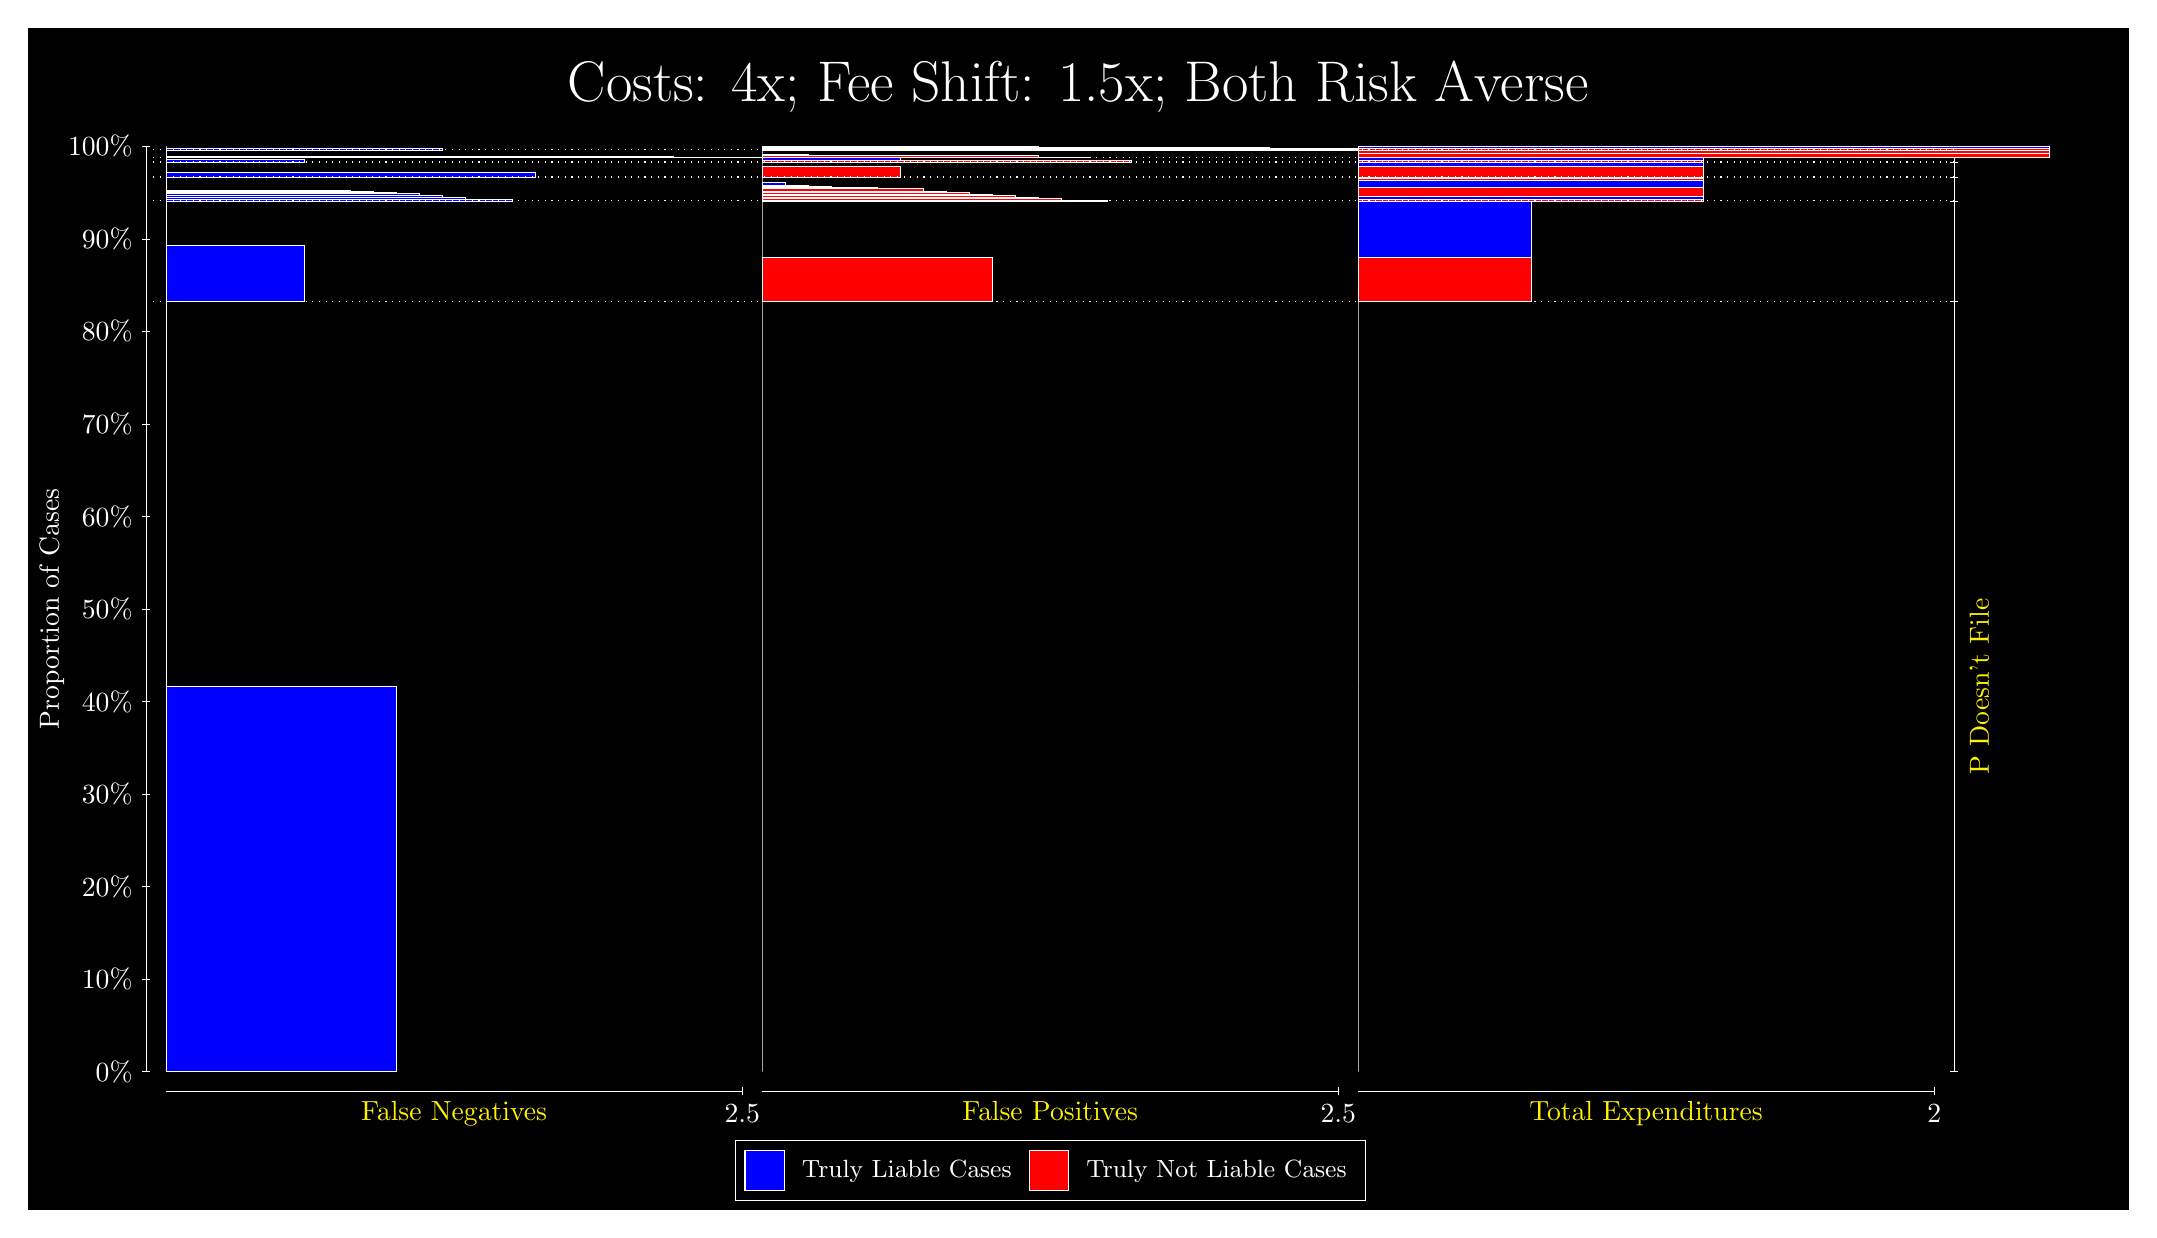
\begin{tikzpicture}
\draw[fill=black] (0,0) rectangle (26.667,15);
\draw[text=white] (0,13.5) rectangle (26.667,15) node[midway] {\huge Costs: 4x; Fee Shift: 1.5x; Both Risk Averse};
\draw[white, very thin] (1.5,1.75) -- (1.5,13.5);
\node[rotate=90, text=white, anchor=center] at (0.3, 7.625) {Proportion of Cases};
\draw[white, very thin] (1.45,1.75) -- (1.55,1.75);
\node[text=white, anchor=east] at (1.45, 1.75) {0\%};
\draw[white, very thin] (1.45,2.925) -- (1.55,2.925);
\node[text=white, anchor=east] at (1.45, 2.925) {10\%};
\draw[white, very thin] (1.45,4.1) -- (1.55,4.1);
\node[text=white, anchor=east] at (1.45, 4.1) {20\%};
\draw[white, very thin] (1.45,5.275) -- (1.55,5.275);
\node[text=white, anchor=east] at (1.45, 5.275) {30\%};
\draw[white, very thin] (1.45,6.45) -- (1.55,6.45);
\node[text=white, anchor=east] at (1.45, 6.45) {40\%};
\draw[white, very thin] (1.45,7.625) -- (1.55,7.625);
\node[text=white, anchor=east] at (1.45, 7.625) {50\%};
\draw[white, very thin] (1.45,8.8) -- (1.55,8.8);
\node[text=white, anchor=east] at (1.45, 8.8) {60\%};
\draw[white, very thin] (1.45,9.975) -- (1.55,9.975);
\node[text=white, anchor=east] at (1.45, 9.975) {70\%};
\draw[white, very thin] (1.45,11.15) -- (1.55,11.15);
\node[text=white, anchor=east] at (1.45, 11.15) {80\%};
\draw[white, very thin] (1.45,12.325) -- (1.55,12.325);
\node[text=white, anchor=east] at (1.45, 12.325) {90\%};
\draw[white, very thin] (1.45,13.5) -- (1.55,13.5);
\node[text=white, anchor=east] at (1.45, 13.5) {100\%};

\draw[white, very thin] (24.457,1.75) -- (24.457,13.5);
\draw[white, very thin] (24.407,1.75) -- (24.507,1.75);
\node[anchor=west] at (24.407, 1.75) {};
\draw[white, very thin] (24.407,11.53) -- (24.507,11.53);
\node[anchor=west] at (24.407, 11.53) {};
\draw[white, very thin] (24.407,12.808) -- (24.507,12.808);
\node[anchor=west] at (24.407, 12.808) {};
\draw[white, very thin] (24.407,13.11) -- (24.507,13.11);
\node[anchor=west] at (24.407, 13.11) {};
\draw[white, very thin] (24.407,13.301) -- (24.507,13.301);
\node[anchor=west] at (24.407, 13.301) {};
\draw[white, very thin] (24.407,13.358) -- (24.507,13.358);
\node[anchor=west] at (24.407, 13.358) {};
\draw[white, very thin] (24.407,13.456) -- (24.507,13.456);
\node[anchor=west] at (24.407, 13.456) {};
\draw[white, very thin] (24.407,13.5) -- (24.507,13.5);
\node[anchor=west] at (24.407, 13.5) {};

\draw[white, very thin, fill=blue] (1.75,1.75) rectangle (4.6775,6.6398);
\draw[white, very thin, fill=red] (1.75,6.6398) rectangle (1.75,11.53);
\draw[white, very thin, fill=blue] (1.75,11.53) rectangle (3.5065,12.243);
\draw[white, very thin, fill=red] (1.75,12.243) rectangle (1.75,12.808);
\draw[white, very thin, fill=blue] (1.75,12.808) rectangle (6.1413,12.824);
\draw[white, very thin, fill=blue] (1.75,12.824) rectangle (5.8486,12.832);
\draw[white, very thin, fill=blue] (1.75,12.832) rectangle (5.5558,12.857);
\draw[white, very thin, fill=blue] (1.75,12.857) rectangle (5.2631,12.879);
\draw[white, very thin, fill=blue] (1.75,12.879) rectangle (4.9703,12.908);
\draw[white, very thin, fill=blue] (1.75,12.908) rectangle (4.6775,12.922);
\draw[white, very thin, fill=blue] (1.75,12.922) rectangle (4.3848,12.934);
\draw[white, very thin, fill=blue] (1.75,12.934) rectangle (4.092,12.94);
\draw[white, very thin, fill=blue] (1.75,12.94) rectangle (3.7993,12.945);
\draw[white, very thin, fill=red] (1.75,12.945) rectangle (1.75,13.11);
\draw[white, very thin, fill=blue] (1.75,13.11) rectangle (6.4341,13.166);
\draw[white, very thin, fill=red] (1.75,13.166) rectangle (1.75,13.301);
\draw[white, very thin, fill=blue] (1.75,13.301) rectangle (3.5065,13.336);
\draw[white, very thin, fill=red] (1.75,13.336) rectangle (1.75,13.358);
\draw[white, very thin, fill=blue] (1.75,13.358) rectangle (13.46,13.363);
\draw[white, very thin, fill=blue] (1.75,13.363) rectangle (8.1906,13.372);
\draw[white, very thin, fill=red] (1.75,13.372) rectangle (1.75,13.456);
\draw[white, very thin, fill=blue] (1.75,13.456) rectangle (5.2631,13.471);
\draw[white, very thin, fill=red] (1.75,13.471) rectangle (1.75,13.484);
\draw[white, very thin, fill=blue] (1.75,13.484) rectangle (1.75,13.5);
\draw[white, very thin, fill=red] (9.3189,1.75) rectangle (9.3189,6.6399);
\draw[white, very thin, fill=blue] (9.3189,6.6399) rectangle (9.3189,11.53);
\draw[white, very thin, fill=red] (9.3189,11.53) rectangle (12.246,12.095);
\draw[white, very thin, fill=blue] (9.3189,12.095) rectangle (9.3189,12.808);
\draw[white, very thin, fill=red] (9.3189,12.808) rectangle (13.71,12.815);
\draw[white, very thin, fill=red] (9.3189,12.815) rectangle (13.417,12.821);
\draw[white, very thin, fill=red] (9.3189,12.821) rectangle (13.125,12.835);
\draw[white, very thin, fill=red] (9.3189,12.835) rectangle (12.832,12.852);
\draw[white, very thin, fill=red] (9.3189,12.852) rectangle (12.539,12.876);
\draw[white, very thin, fill=red] (9.3189,12.876) rectangle (12.246,12.894);
\draw[white, very thin, fill=red] (9.3189,12.894) rectangle (11.954,12.922);
\draw[white, very thin, fill=red] (9.3189,12.922) rectangle (11.661,12.935);
\draw[white, very thin, fill=red] (9.3189,12.935) rectangle (11.368,12.973);
\draw[white, very thin, fill=blue] (9.3189,12.973) rectangle (10.783,12.979);
\draw[white, very thin, fill=blue] (9.3189,12.979) rectangle (10.49,12.984);
\draw[white, very thin, fill=blue] (9.3189,12.984) rectangle (10.197,12.996);
\draw[white, very thin, fill=blue] (9.3189,12.996) rectangle (9.9044,13.01);
\draw[white, very thin, fill=blue] (9.3189,13.01) rectangle (9.6116,13.039);
\draw[white, very thin, fill=blue] (9.3189,13.039) rectangle (9.3189,13.11);
\draw[white, very thin, fill=red] (9.3189,13.11) rectangle (11.075,13.245);
\draw[white, very thin, fill=blue] (9.3189,13.245) rectangle (9.3189,13.301);
\draw[white, very thin, fill=red] (9.3189,13.301) rectangle (14.003,13.324);
\draw[white, very thin, fill=blue] (9.3189,13.324) rectangle (11.075,13.358);
\draw[white, very thin, fill=red] (9.3189,13.358) rectangle (12.832,13.392);
\draw[white, very thin, fill=blue] (9.3189,13.392) rectangle (9.9044,13.401);
\draw[white, very thin, fill=red] (9.3189,13.401) rectangle (9.3189,13.452);
\draw[white, very thin, fill=blue] (9.3189,13.452) rectangle (9.3189,13.456);
\draw[white, very thin, fill=red] (9.3189,13.456) rectangle (21.029,13.459);
\draw[white, very thin, fill=blue] (9.3189,13.459) rectangle (18.102,13.475);
\draw[white, very thin, fill=red] (9.3189,13.475) rectangle (15.759,13.486);
\draw[white, very thin, fill=blue] (9.3189,13.486) rectangle (12.832,13.5);
\draw[white, very thin, fill=red] (16.888,1.75) rectangle (16.888,6.6399);
\draw[white, very thin, fill=blue] (16.888,6.6399) rectangle (16.888,11.53);
\draw[white, very thin, fill=red] (16.888,11.53) rectangle (19.083,12.095);
\draw[white, very thin, fill=blue] (16.888,12.095) rectangle (19.083,12.808);
\draw[white, very thin, fill=red] (16.888,12.808) rectangle (21.279,12.833);
\draw[white, very thin, fill=blue] (16.888,12.833) rectangle (21.279,12.863);
\draw[white, very thin, fill=red] (16.888,12.863) rectangle (21.279,12.983);
\draw[white, very thin, fill=blue] (16.888,12.983) rectangle (21.279,13.072);
\draw[white, very thin, fill=red] (16.888,13.072) rectangle (21.279,13.092);
\draw[white, very thin, fill=blue] (16.888,13.092) rectangle (21.279,13.11);
\draw[white, very thin, fill=red] (16.888,13.11) rectangle (21.279,13.245);
\draw[white, very thin, fill=blue] (16.888,13.245) rectangle (21.279,13.301);
\draw[white, very thin, fill=red] (16.888,13.301) rectangle (21.279,13.324);
\draw[white, very thin, fill=blue] (16.888,13.324) rectangle (21.279,13.358);
\draw[white, very thin, fill=red] (16.888,13.358) rectangle (25.67,13.409);
\draw[white, very thin, fill=blue] (16.888,13.409) rectangle (25.67,13.414);
\draw[white, very thin, fill=red] (16.888,13.414) rectangle (25.67,13.448);
\draw[white, very thin, fill=blue] (16.888,13.448) rectangle (25.67,13.456);
\draw[white, very thin, fill=red] (16.888,13.456) rectangle (25.67,13.469);
\draw[white, very thin, fill=blue] (16.888,13.469) rectangle (25.67,13.5);
\draw[white, dotted] (1.5,11.53) -- (24.457,11.53);
\draw[white, dotted] (1.5,12.808) -- (24.457,12.808);
\draw[white, dotted] (1.5,13.11) -- (24.457,13.11);
\draw[white, dotted] (1.5,13.301) -- (24.457,13.301);
\draw[white, dotted] (1.5,13.358) -- (24.457,13.358);
\draw[white, dotted] (1.5,13.456) -- (24.457,13.456);
\draw[white, very thin] (1.75,1.5) -- (9.0689,1.5);
\node[text=yellow, anchor=north] at (5.4094, 1.5) {False Negatives};
\draw[white, very thin] (9.0689,1.45) -- (9.0689,1.55);
\node[text=white, anchor=north] at (9.0689, 1.45) {2.5};

\draw[white, very thin] (9.3189,1.5) -- (16.638,1.5);
\node[text=yellow, anchor=north] at (12.978, 1.5) {False Positives};
\draw[white, very thin] (16.638,1.45) -- (16.638,1.55);
\node[text=white, anchor=north] at (16.638, 1.45) {2.5};

\draw[white, very thin] (16.888,1.5) -- (24.207,1.5);
\node[text=yellow, anchor=north] at (20.547, 1.5) {Total Expenditures};
\draw[white, very thin] (24.207,1.45) -- (24.207,1.55);
\node[text=white, anchor=north] at (24.207, 1.45) {2};

\node[text=yellow, centered, rotate=90] at (24.777, 6.6399) {P Doesn't File};







\draw (12.978300999999998,1.5) node[draw=none] (baseCoordinate) {};
\begin{scope}[align=center]
        \matrix[scale=0.5, draw=white, below=0.5cm of baseCoordinate, nodes={draw}, column sep=0.1cm]{
            \node[rectangle, draw, minimum width=0.5cm, minimum height=0.5cm, fill=blue] {}; &
            \node[draw=none, font=\small, text=white] (B) {Truly Liable Cases}; &
            \node[rectangle, draw, minimum width=0.5cm, minimum height=0.5cm, fill=red] {}; &
            \node[draw=none, font=\small, text=white] (B) {Truly Not Liable Cases}; \\
            };
\end{scope}

\end{tikzpicture}
\end{document}